\documentclass{beamer}

\mode<presentation>
{
  \usetheme{CambridgeUS}      % or try Darmstadt, Madrid, ...
  \usecolortheme{default} % or try albatross, beaver, crane, ...
  \usefonttheme{default}  % or try serif, structurebold, ...
  \setbeamertemplate{navigation symbols}{}
  \setbeamertemplate{caption}[numbered]
} 

\usepackage[english]{babel}
\usepackage[utf8x]{inputenc}
\usepackage{listings}
\usepackage[ampersand]{easylist}



\definecolor{KTI_green}{RGB}{150, 189, 13}
\definecolor{TU_red}{RGB}{255, 55, 81}
\definecolor{faint_gray}{RGB}{180, 180, 180}

\definecolor{syntax_green}{rgb}{0,0.6,0}
\definecolor{syntax_gray}{rgb}{0.9, 0.9, 0.9}
\definecolor{syntax_mauve}{rgb}{0.58,0,0.82}

\lstset{ 
  backgroundcolor=\color{syntax_gray},  % choose the background color
  basicstyle=\scriptsize\ttfamily,        		% size of fonts used for the code
  breaklines=false,                		% automatic line breaking only at whitespace
  captionpos=b,                    		% sets the caption-position to bottom
  commentstyle=\color{syntax_green},    % comment style
  escapeinside={\%*}{*)},          		% if you want to add LaTeX within your code
  keywordstyle=\color{blue},       		% keyword style
  stringstyle=\color{syntax_mauve},     % string literal style
  columns=fullflexible,
  frame=single,
  framesep=0.5cm,
  framexleftmargin=0.5cm,
  xleftmargin=0.5cm,
  framexrightmargin=0.5cm,
  xrightmargin=0.5cm,
  frame=tb,                 
    numbers=left,                    
    numbersep=15pt,  
  }
  
  
\newcommand{\logopython}{\raggedleft 
\includegraphics[height=0.5cm]{logo_python}\hspace{0.1cm}\\\raggedright}
\newcommand{\logopythonbottom}{\raggedleft\vspace{-0.8cm}
\includegraphics[height=0.5cm]{logo_python}\hspace*{0.05cm}\\\raggedright}

\title[BSP30 - Supermarkt]{Supermarkt}
\author{Dickbauer Y., Moser P., Perner M.}
\institute{PS Computergestützte Modellierung, WS 2016/17}
%\date{Date of Presentation}

\begin{document}

\begin{frame}
  \titlepage
\end{frame}

\begin{frame}{Outline}
  \tableofcontents
\end{frame}

\section{Aufgabenstellung}
\begin{frame}{Aufgabenstellung}
In einem Supermarkt gibt es derzeit zwei Kassen, die für alle Kunden zuständig ist. Da es etliche Kunden gibt, die nur wenige Waren kaufen, ist die Geschäftsführung am überlegen, eine dritte Kasse als Expresskasse einzuführen, um die Warteschlange zu verringern. Die Expresskasse ist nur für jene Kunden offen, die weniger als 5 Waren einkaufen.
\\~\\
Die Ankunftsrate für normale Kunden ist exponentialverteilt mit Erwartungswert von 3 Minuten, die Ankunftsrate von "Expresskunden" ist exponentialverteilt mit Erwartungswert von 5 Minuten. Die Bedienzeit von normalen Kunden ist exponentialverteilt mit Erwartungswert von 5 Minuten, die von "Expresskunden" ist ebenso exponentialverteilt mit Erwartungswert von 3 Minuten.
\end{frame}

\begin{frame}{Aufgabenstellung}
Wie verändern sich die mittleren Schlangenlängen der einzelnen Kassen bei den unterschiedlichen Strategien?
\vspace{1cm}
\begin{itemize}
  \item Eingabe: -
  \item Output: Warteschlangenlänge am Periodenanfang je Kassa, Neuankunft und Typ, Abfertigung in Periode, sowie die oben angeführten Kennzahlen
\end{itemize}
\end{frame}

\section{Flow Chart}
\begin{frame}{Flow Chart}
	\centering
  	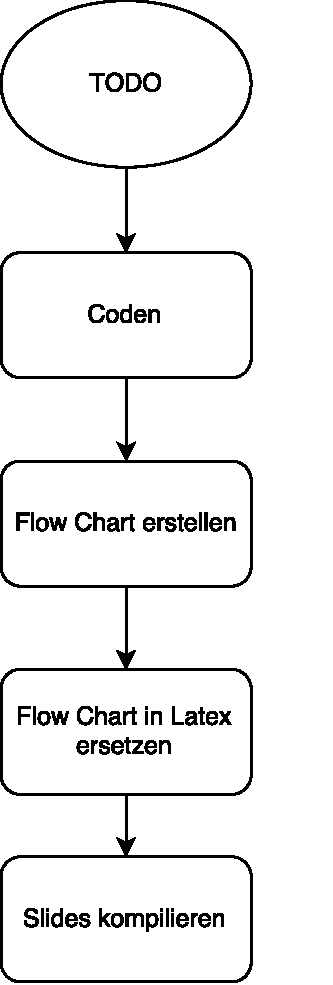
\includegraphics[scale=0.3]{FlowChartTodo.pdf}
\end{frame}

\subsection{Verwendete Funktionen}
%\begin{frame}[fragile]{Funktion loaded\_random\_choice(..)}
  \begin{itemize}
    \item Diese Funktion verlangt eine WSKL Liste als Eingabeparameter
    \item Gibt einen Index zurück, welcher 0 bis $\left\vert{probality\_list}\right\vert-1$ sein kann.
    \item Diese Indizes haben eine gewichtete WSKL, welche jeweils an der Position in der Eingabeliste steht
    \item Beispiel probility\_list := [ 0.9, 0.1 ]  $\Rightarrow$ mit p=90\% wird 0 zurückgegeben, p=10\% für 1
  \end{itemize}
  \begin{lstlisting}[language=python]
def loaded_random_choice(probability_list):
    n = len(probability_list)
    random_number = random.random()
    cum_p = 0
    for i in range(n):
        cum_p += probability_list[i]
        if cum_p > random_number:
            return i
    return None
\end{lstlisting}
\logopythonbottom
\end{frame}	

\section{Ergebnisse}
\begin{frame}[fragile]{Simulationsergebnis Var 1, 2 Normale Kassen}
    	\begin{figure}[h!]
    	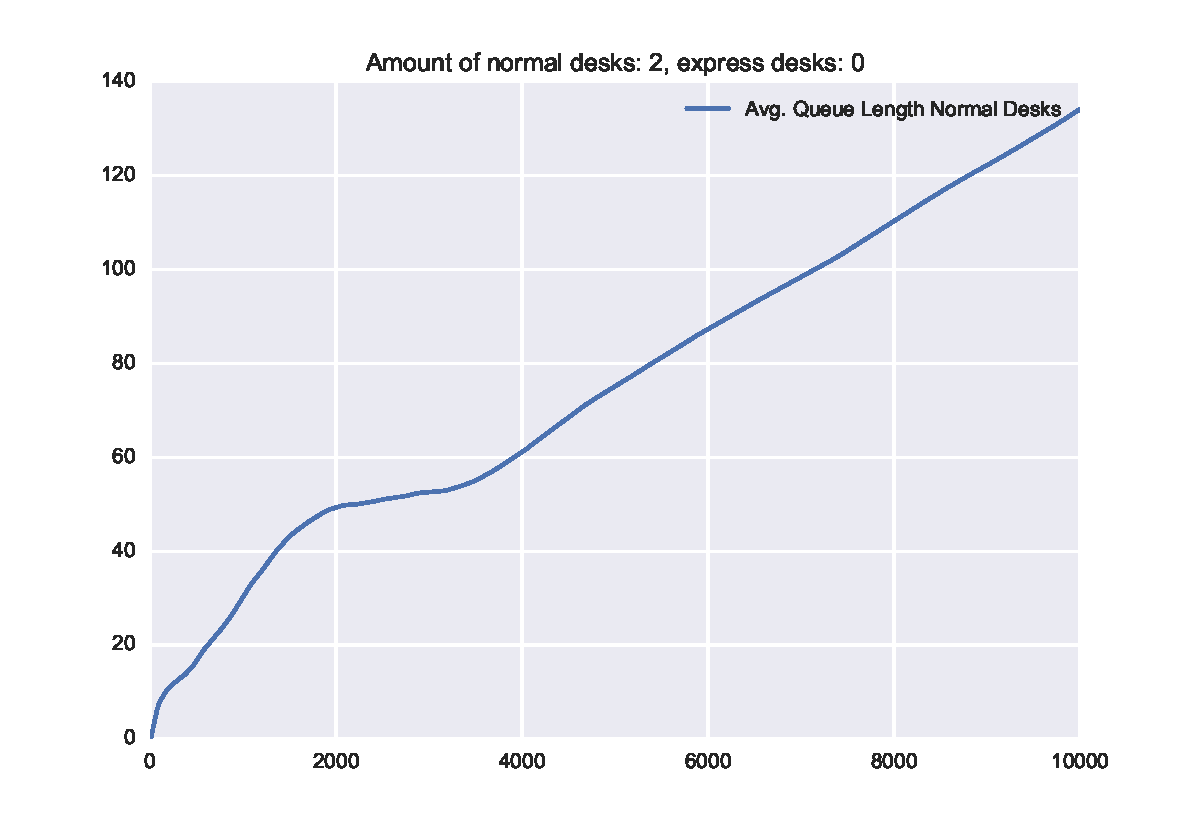
\includegraphics[scale=0.5]{BSP30_Plot_1.pdf}
		\end{figure}
\end{frame}

\begin{frame}[fragile]{Simulationsergebnis Var 2, 2 Normale Kassen und 1 Expresskassa}
    	\begin{figure}[h!]
    	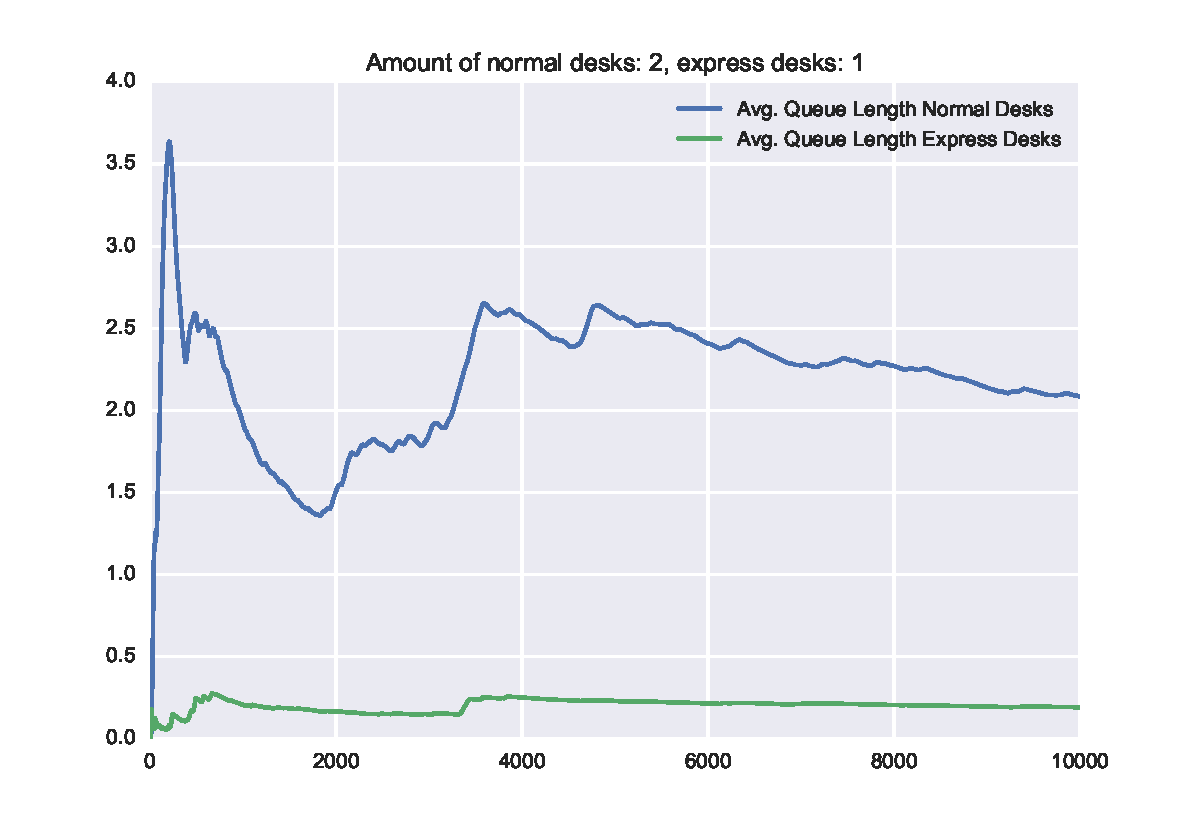
\includegraphics[scale=0.5]{BSP30_Plot_2.pdf}
		\end{figure}
\end{frame}

\begin{frame}[fragile]{Simulationsergebnis Var 3, 3 Normale Kassen und 0 Expresskassa}
    	\begin{figure}[h!]
    	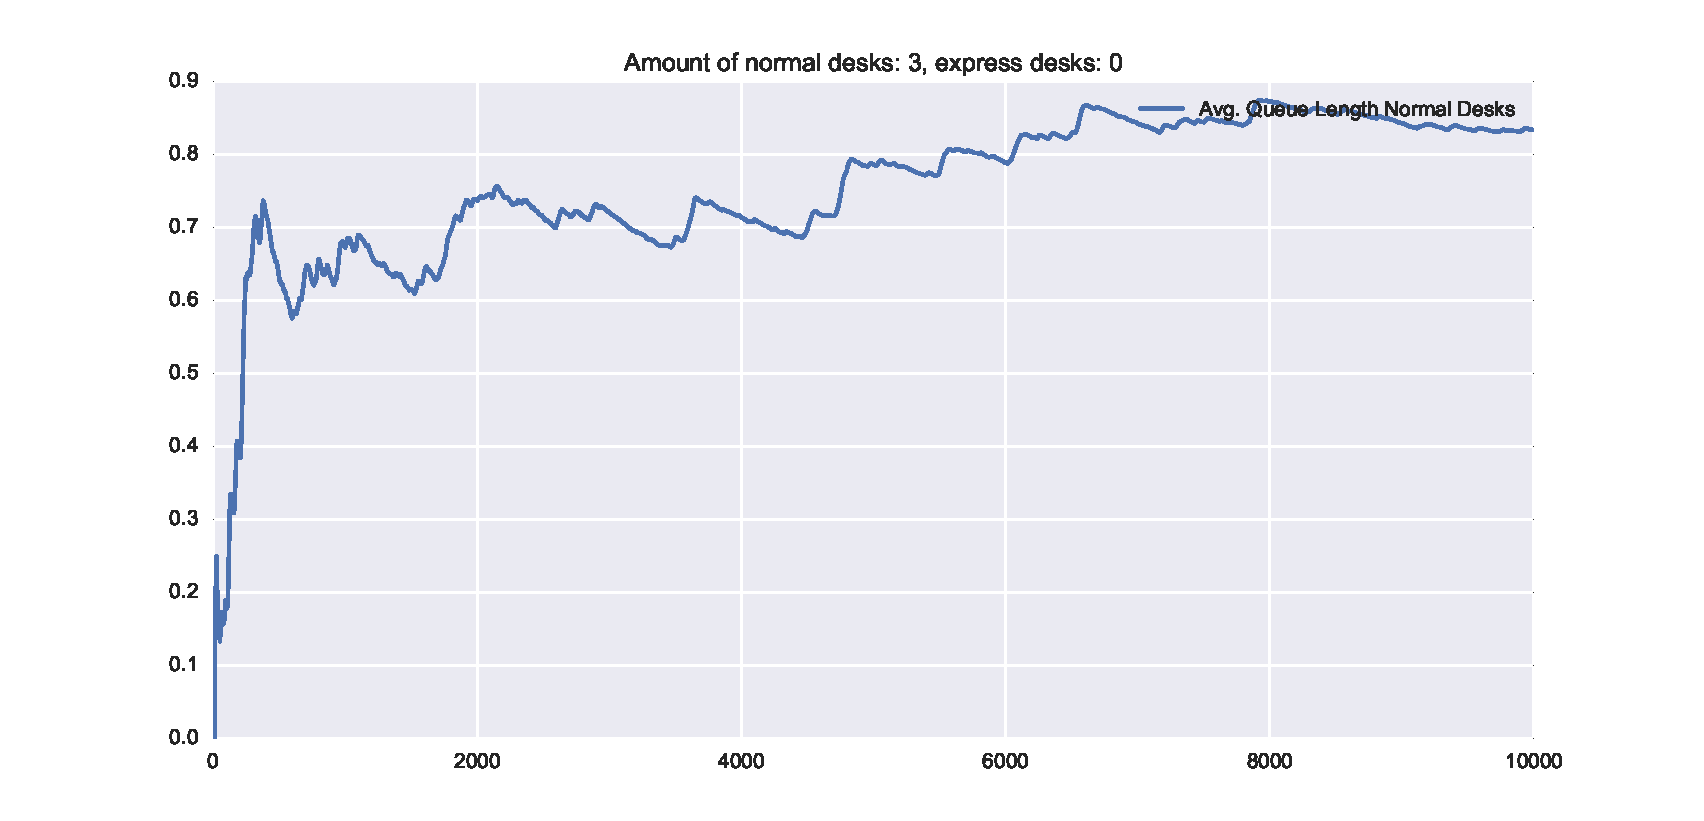
\includegraphics[scale=0.4]{BSP30_Plot_3.pdf}
		\end{figure}
\end{frame}

\end{document}
